%% abtex2-modelo-slides.tex, v-1.0 gfabinhomat
%% Copyright 2012-2016 by abnTeX2 group at http://www.abntex.net.br/ 
%%
%% This work may be distributed and/or modified under the
%% conditions of the LaTeX Project Public License, either version 1.3
%% of this license or (at your option) any later version.
%% The latest version of this license is in
%%   http://www.latex-project.org/lppl.txt
%% and version 1.3 or later is part of all distributions of LaTeX
%% version 2005/12/01 or later.
%%
%% This work has the LPPL maintenance status `maintained'.
%% 
%% The Current Maintainer of this work is Fábio Rodrigues Silva, 
%% member of abnTeX2 team, led by Lauro César Araujo. 
%% Further information are available on 
%% http://www.abntex.net.br/
%%
%% This work consists of the files abntex2-modelo-slides.tex, 
%% abntex2-modelo-references.bib and abntex2-modelo-marca.pdf
%%
%% Modelo desenvolvido por Fábio Rodrigues Silva (gfabinhomat@gmail.com)
%% Mais informações podem ser obtidas no guia do usuário Beamer 
%% (http://linorg.usp.br/CTAN/macros/latex/contrib/beamer/doc/beameruserguide.pdf)
%% Informações rápidas podem ser acessadas em http://en.wikibooks.org/wiki/LaTeX/Presentations

\PassOptionsToPackage{dvipsnames}{xcolor}

% Apresentações em widescreen. Outros valores possíveis: 1610, 149, 54, 43 e 32.
% Por padrão, as apresentações são no formato 4:3 (sem o aspectratio).
\documentclass[aspectratio=169]{beamer}	 	

\usepackage{svg}
\usepackage{diagbox}
\svgpath{{img/}}

\usetheme{Pittsburgh}
\usecolortheme{default}
\usefonttheme[onlymath]{serif}			% para fontes matemáticas
% Enconte mais temas e cores em http://www.hartwork.org/beamer-theme-matrix/ 
% Veja também http://deic.uab.es/~iblanes/beamer_gallery/index.html

% Customizações de Cores: fg significa cor do texto e bg é cor do fundo
\setbeamercolor{normal text}{fg=black}
\setbeamercolor{alerted text}{fg=red}
\setbeamercolor{author}{fg=black}
\setbeamercolor{institute}{fg=black}
\setbeamercolor{date}{fg=OliveGreen}
\setbeamercolor{frametitle}{fg=OliveGreen}
\setbeamercolor{framesubtitle}{fg=OliveGreen}
\setbeamercolor{block title}{bg=OliveGreen, fg=white}		%Cor do título
\setbeamercolor{block body}{bg=lightgray, fg=darkgray}	%Cor do texto (bg= fundo; fg=texto)

% ---
% PACOTES
% ---
\usepackage[alf]{abntex2cite}		% Citações padrão ABNT
\usepackage[brazil]{babel}		% Idioma do documento
\usepackage{color}			% Controle das cores
\usepackage[T1]{fontenc}		% Selecao de codigos de fonte.
\usepackage{graphicx}			% Inclusão de gráficos
\usepackage[utf8]{inputenc}		% Codificacao do documento (conversão automática dos acentos)
\usepackage{txfonts}			% Fontes virtuais
% ---

% --- Informações do documento ---
\title{Desenvolvimento de um subsistema de comunicação utilizando tecnologia LoRa aplicado a pequenos satélites.}
\author{Lucas Saavedra Vaz}
\institute{Universidade Federal de São Paulo
	    \par
	    Instituto de Ciência e Tecnologia}
\date{20 de Janeiro de 2023}
% ---

% ----------------- INÍCIO DO DOCUMENTO --------------------------------------
\begin{document}

% ----------------- NOVO SLIDE --------------------------------
\begin{frame}

\begin{minipage}{1\linewidth}
  \centering
  \begin{tabular}{cc}
    \begin{tabular}{c}
      
\includegraphics[width=3.0cm]{img/Unifesp.png}
    \end{tabular}
    &
    \begin{tabular}{c}
      \textbf{Universidade Federal de São Paulo} \\ \textbf{Instituto de Ciência e Tecnologia}
    \end{tabular}
  \end{tabular}
\end{minipage}

\titlepage

\end{frame}

% ----------------- NOVO SLIDE --------------------------------
\begin{frame}{Sumário}
\tableofcontents
\end{frame}

% ----------------- NOVO SLIDE --------------------------------
\section{Introdução}

\begin{frame}{Introdução}

\begin{itemize}
    \item Satélites são dispositivos em orbita com um propósito;
    \item Dispositivos de grande porte possuem um custo elevado;
    \item Miniaturização;
    \item Plataforma e carga útil;
    \item Diversos métodos de modulação de rádio são utilizadas;
    \item LoRa é um dos métodos mais populares.
\end{itemize}

\end{frame}

% ----------------- NOVO SLIDE --------------------------------
\section{Objetivos}

\begin{frame}
\frametitle{Objetivos}

Objetivos do desenvolvimento do trabalho:

\begin{itemize}
    \item Utilizar microcontroladores para testes de transmissões LoRa;
    \item Analisar e implementar as possíveis configurações de transmissão;
    \item Aplicar recursos de software para tornar a transmissão mais confiável;
    \item Produzir um \emph{framework} para selecionar diferentes parâmetros de LoRa com base nos requisitos do projeto;
\end{itemize}

\end{frame}

% ----------------- NOVO SLIDE --------------------------------
\section{Fundamentação Teórica}

\begin{frame}
\frametitle{Fundamentação Teórica}
\framesubtitle{CubeSats}

\begin{itemize}
    \item 10 cm x 10 cm x 10 cm e 1,33 kg;
    \item Grandes vantagens em relação a satélites de grande porte;
    \item Rideshare.
\end{itemize}

\begin{figure}
  \centering
  \includegraphics[scale=0.12]{img/Cubesat.jpg}
  \caption{PhoneSat 2.5. Fonte: \citeonline{thompson_2015}}
\end{figure}

\end{frame}

% ----------------- NOVO SLIDE --------------------------------
\begin{frame}
\frametitle{Fundamentação Teórica}
\framesubtitle{CubeSats}

\begin{figure}
  \centering
  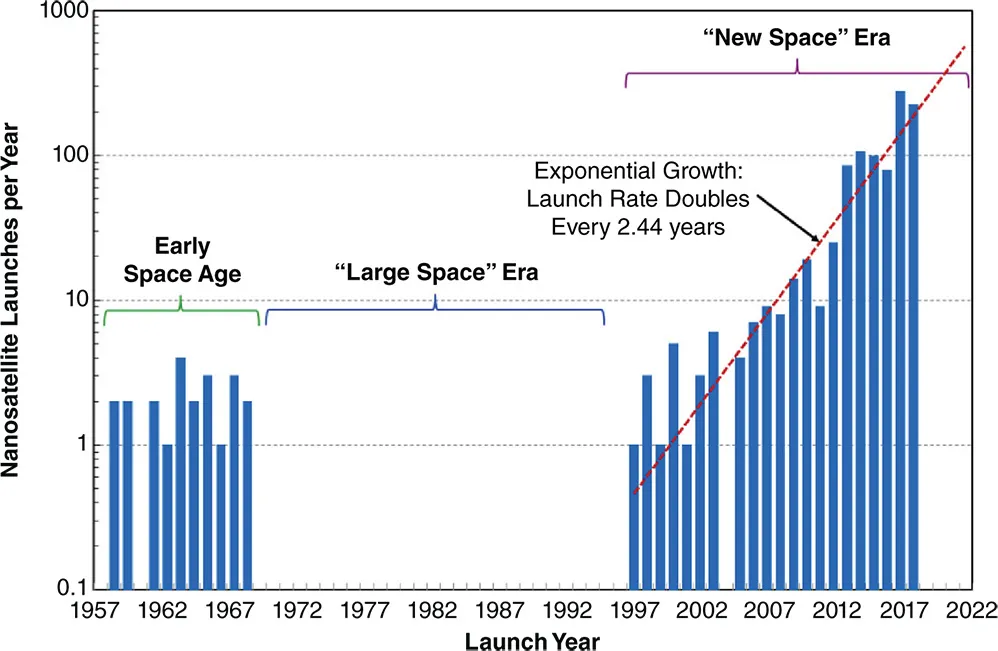
\includegraphics[scale=0.25]{img/Launches.png}
  \caption{Lançamentos de nanossatélites por ano. Fonte: \citeonline{carvalho_2020}}
\end{figure}

\end{frame}

% ----------------- NOVO SLIDE --------------------------------
\begin{frame}

\frametitle{Fundamentação Teórica}
\framesubtitle{Sistemas Embarcados}

\begin{itemize}
    \item Sistemas computacionais de pequeno porte;
    \item Função estática dentro de um dispositivo.
\end{itemize}

\begin{figure}
  \centering
  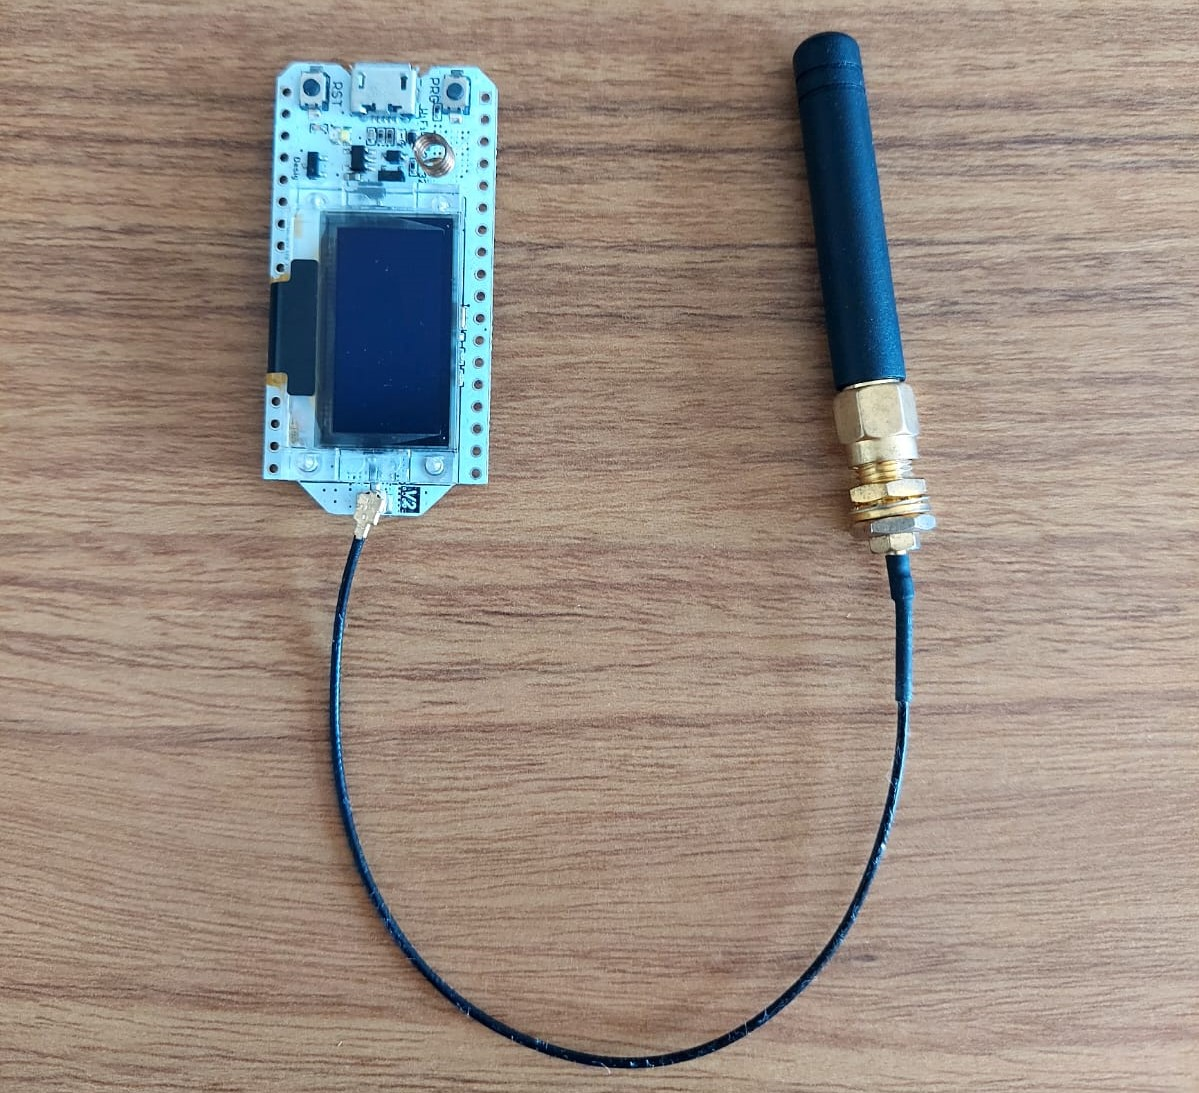
\includegraphics[scale=0.16]{img/HW.jpg}
  \caption{ESP32 WiFi LoRa V2.}
\end{figure}

\end{frame}

% ----------------- NOVO SLIDE --------------------------------
\begin{frame}

\frametitle{Fundamentação Teórica}
\framesubtitle{LoRa}

\begin{itemize}
    \item Modulação baseada em \emph{chirps};
    \item Baixa potência e longo alcance;
    \item Melhor utilizado em situações onde a perda de pacotes e velocidade de transmissão não é de extrema importância;
    \item Principais parâmetros de configuração disponíveis:
    \begin{itemize}
        \item Potência de Transmissão (\emph{TX Power});
        \item Largura de Banda (BW);
        \item Fator de Espalhamento (SF);
        \item Razão de Codificação (CR).
    \end{itemize}
    
\end{itemize}

\end{frame}

% ----------------- NOVO SLIDE --------------------------------
\begin{frame}

\frametitle{Fundamentação Teórica}
\framesubtitle{LoRa}

\begin{figure}
  \centering
  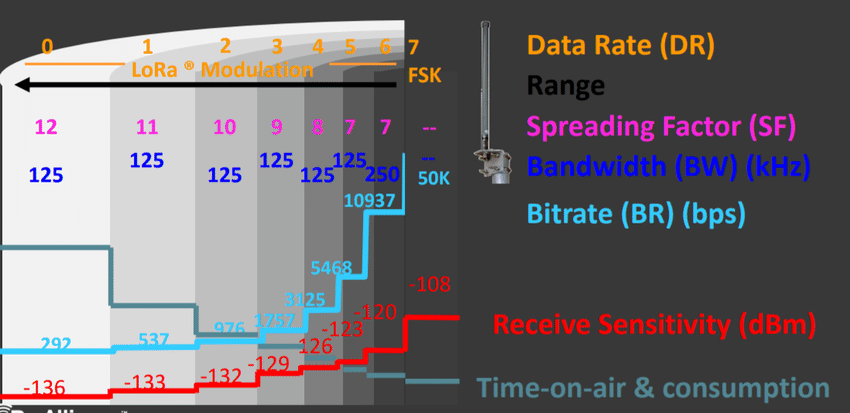
\includegraphics[scale=0.4]{img/Sens.png}
  \caption{Relação entre os parâmetros LoRa. Fonte: \citeonline{alliance_2017}}
\end{figure}

\end{frame}

% ----------------- NOVO SLIDE --------------------------------
\begin{frame}

\frametitle{Fundamentação Teórica}
\framesubtitle{Códigos Corretores de Erros}

\begin{itemize}
    \item Algoritmos capazes de recuperar informação perdida a partir de redundância;
    \item Informação adicionada a cada "palavra".
\end{itemize}

\begin{figure}
  \centering
  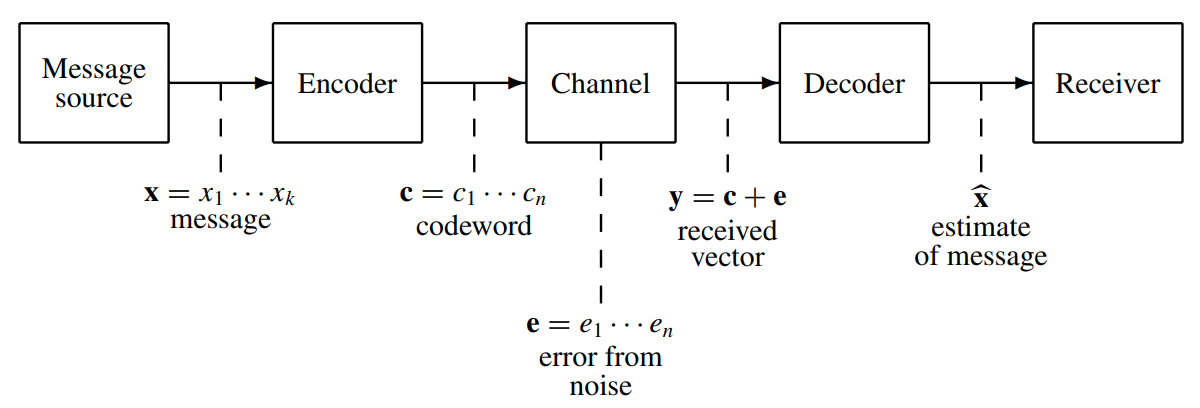
\includegraphics[scale=0.35]{img/Comm.png}
  \caption{Modelo de canal de comunicação. Fonte: \citeonline{huffman_2010}}
\end{figure}

\end{frame}

% ----------------- NOVO SLIDE --------------------------------
\section{Desenvolvimento}

\begin{frame}

\frametitle{Desenvolvimento}
\framesubtitle{Hardware}

\begin{itemize}
    \item SX1276 operando na frequência de 915 MHz \cite{anatel_2017};
    \item Antena de baixo ganho;
    \item Os sistemas podem diferir desde que utilizem os mesmos parâmetros.
\end{itemize}

\begin{figure}
  \centering
  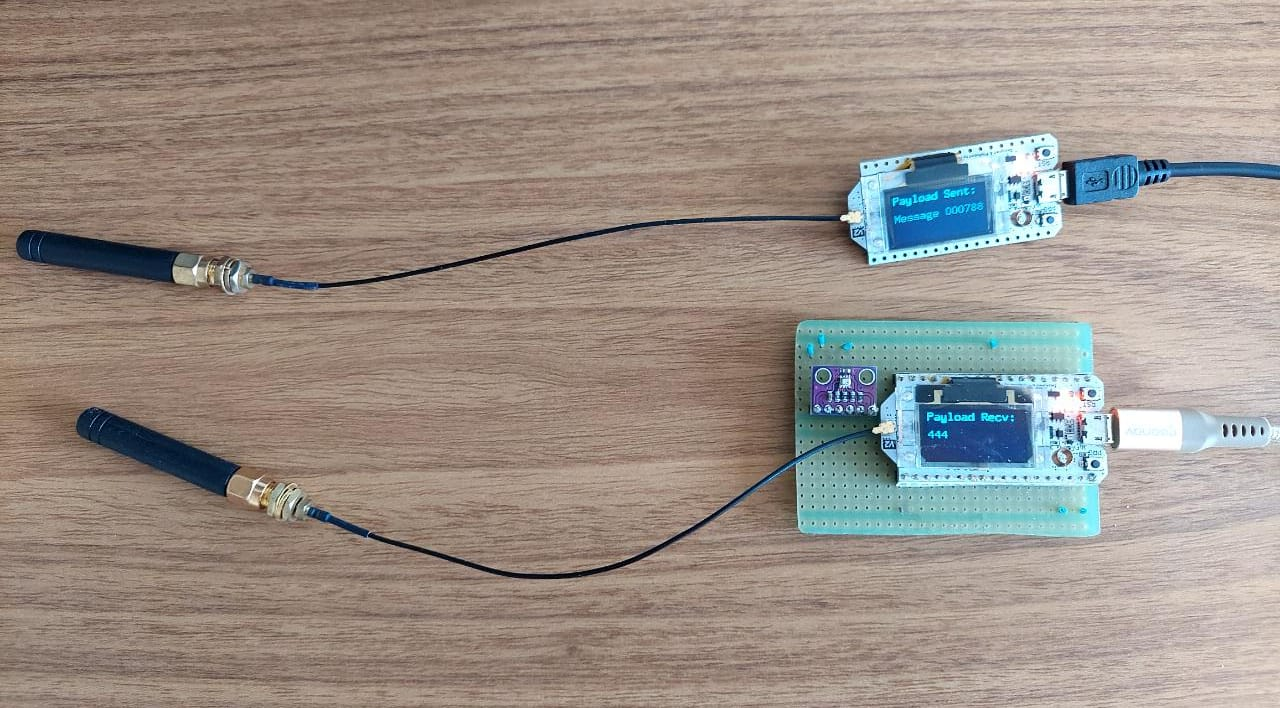
\includegraphics[scale=0.15]{img/Test.jpg}
  \caption{Transmissor e receptor utilizados nos testes.}
\end{figure}

\end{frame}

% ----------------- NOVO SLIDE --------------------------------
\begin{frame}

\frametitle{Desenvolvimento}
\framesubtitle{Software}

\begin{itemize}
    \item Arduino IDE (C++);
    \item Mensgens de teste de 23 bytes;
    \item Camada dupla de correção de erros \cite{yazdani_2021};
    \item Parâmetros de rádio controlados por \emph{software}.
\end{itemize}

\begin{figure}
  \centering
  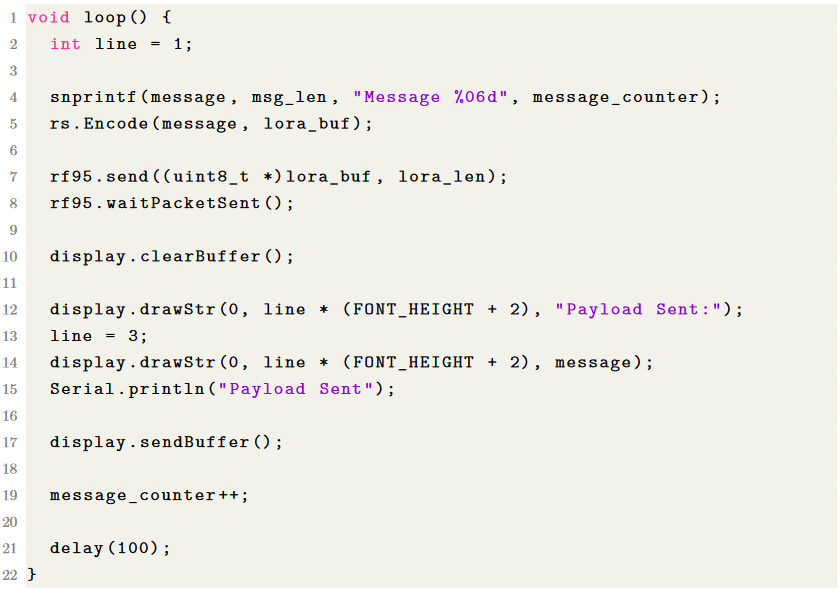
\includegraphics[scale=0.25]{img/Code.png}
  \caption{Construção e codificação do pacote a ser transmitido.}
\end{figure}

\end{frame}

% ----------------- NOVO SLIDE --------------------------------
\begin{frame}

\frametitle{Desenvolvimento}
\framesubtitle{Testes}

\begin{itemize}
    \item Teste de distância máxima, taxa de sucesso e tempo de transmissão;
    \item Combinação dos parâmetros testados:
    \begin{itemize}
        \item Largura de banda (BW): 125MHz e 250MHz;
        \item Fator de espalhamento (SF): 7 a 12;
        \item Razão de Codificação (CR): 1 e 4.
    \end{itemize}
\end{itemize}

\begin{figure}
  \centering
  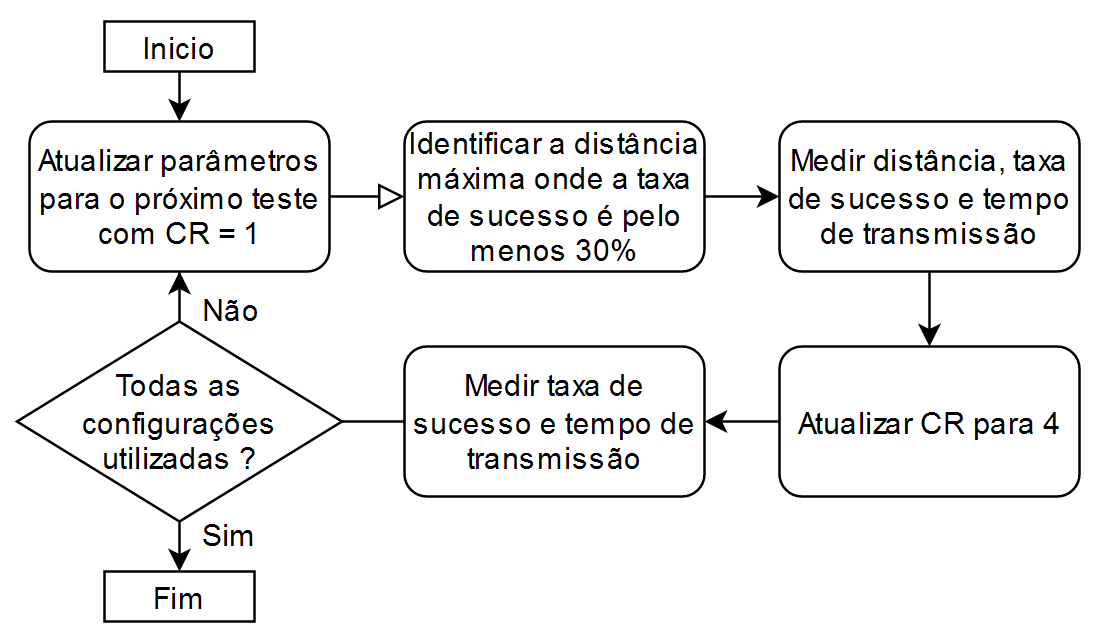
\includegraphics[scale=0.23]{img/Flux.png}
  \caption{Fluxo de testes.}
\end{figure}

\end{frame}

% ----------------- NOVO SLIDE --------------------------------
\section{Resultados}

\begin{frame}

\frametitle{Resultados}
\framesubtitle{Distância Máxima}

\begin{itemize}
    \item Diferença inicial entre as curvas;
    \item Declive superior na curva de 125MHz.
\end{itemize}

\begin{figure}
  \centering
  \includesvg[scale=0.45]{img/Dist.svg}
  \caption{Distâncias máximas entre largura de banda de 125 e 250 MHz.}
\end{figure}

\end{frame}

% ----------------- NOVO SLIDE --------------------------------
\begin{frame}

\frametitle{Resultados}
\framesubtitle{Taxa de sucesso de transmissão}

\begin{itemize}
    \item 125MHz: Ganho médio de 14,7\% e máximo de 45\%;
    \item 250MHz: Ganho médio de 7\% e máximo de 31\%.
\end{itemize}

\begin{figure}
  \centering
  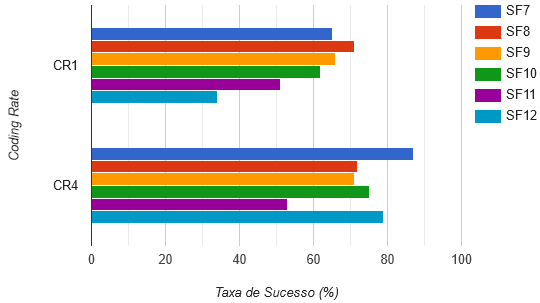
\includegraphics[width=0.475\textwidth]{img/CR125.png}
  \hfill
  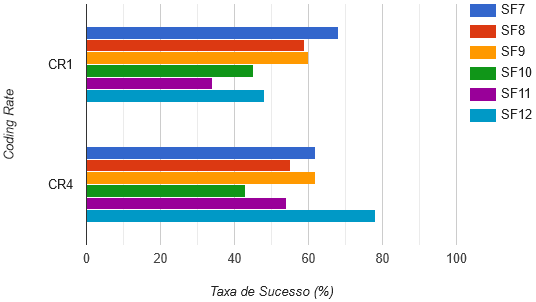
\includegraphics[width=0.475\textwidth]{img/CR250.png}
  \caption{Taxa de sucesso com largura de banda de 125MHz (esquerda) e 250MHz (direita).}
\end{figure}

\end{frame}

% ----------------- NOVO SLIDE --------------------------------
\begin{frame}

\frametitle{Resultados}
\framesubtitle{Tempo de transmissão}

\begin{itemize}
    \item Maior tempo de transmissão implica em maior gasto de energia;
    \item Importante em dispositivos com fonte de energia limitadas;
\end{itemize}

\begin{figure}
  \centering
  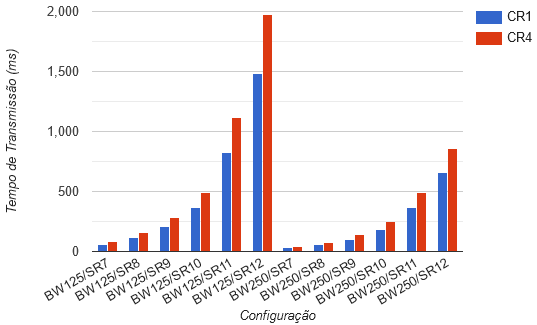
\includegraphics[scale=0.55]{img/Time.png}
  \caption{Tempo de transmissão de mensagem de 23 bytes em diferentes configurações LoRa.}
\end{figure}

\end{frame}

% ----------------- NOVO SLIDE --------------------------------
\begin{frame}

\frametitle{Resultados}
\framesubtitle{Síntese}

\begin{itemize}
    \item +: Aumentar o parâmetro melhora a característica;
    \item -: Diminuir o parâmetro melhora a característica;
    \item $\alpha$: Caso a perda de dados não tenha consequências, é ideal escolher o menor SF possível que atenda a distância desejada;
    \item $\beta$: Não altera a característica em si, porém torna a conexão mais consistente.
\end{itemize}

\begin{table}[]
\centering
\caption{Configuração de parâmetros para diferentes características desejadas}
\begin{tabular}{|l|c|c|c|c|} 
\hline
\backslashbox{Característica}{Parâmetro} & \multicolumn{1}{l|}{BW} & \multicolumn{1}{l|}{SF} & \multicolumn{1}{l|}{CR} & \multicolumn{1}{l|}{Potência de Transmissão}  \\ 
\hline
Distância & - & + & $\beta$ & + \\ 
\hline
Robustez & + & $\alpha$ & + & + \\ 
\hline
\textit{Bitrate} & + & - & - & + \\ 
\hline
Eficiência energética & + & - & - & - \\
\hline
\end{tabular}
\end{table}

\end{frame}

% ----------------- NOVO SLIDE --------------------------------
\section{Conclusão}

\begin{frame}

\frametitle{Conclusão}

\begin{itemize}
    \item Atestamos que LoRa é viável para a comunicação com satélites de pequeno porte;
    \item Parâmetros LoRa dependerão do projeto;
    \item Melhorias futuras:
    \begin{itemize}
        \item Validação em ambiente controlado (câmara anecoica);
        \item Antena de maior qualidade e ganho;
        \item Utilização de RTOS.
    \end{itemize}
\end{itemize}

\end{frame}

% ----------------- NOVO SLIDE --------------------------------
\section{Referências}

% --- O comando \allowframebreaks ---
% Se o conteúdo não se encaixa em um quadro, a opção allowframebreaks instrui 
% beamer para quebrá-lo automaticamente entre dois ou mais quadros,
% mantendo o frametitle do primeiro quadro (dado como argumento) e acrescentando 
% um número romano ou algo parecido na continuação.

\begin{frame}[allowframebreaks]{Referências}
\bibliography{bibliografia}
\end{frame}

% ----------------- FIM DO DOCUMENTO -----------------------------------------
\end{document}
